\problemname{\problemyamlname}

La grande ville de Karwa-sur-mer souhaite moderniser les buildings présents sur la digue.
En effet, la ville veut poser des panneaux solaires sur ceux-ci et, afin de profiter un maximum de la production électrique de ceux-ci, elle décide de recouvrir bien évidemment les toits des bâtiments et les façades de côtés.

Pour cela, vous êtes engagé afin de déterminer combien de mètres de panneaux la ville aura besoin pour équiper ses bâtiments.
La ville vous donne pour cela un plan en vue de face de la digue vous spécifiant la taille des bâtiments comme ceci :

Pour chaque emplacement de 1 mètre de large, le plan vous donne la hauteur du bâtiment à cet emplacement comme illustré par la figure ci-dessous.

\begin{figure}[h]
\centering
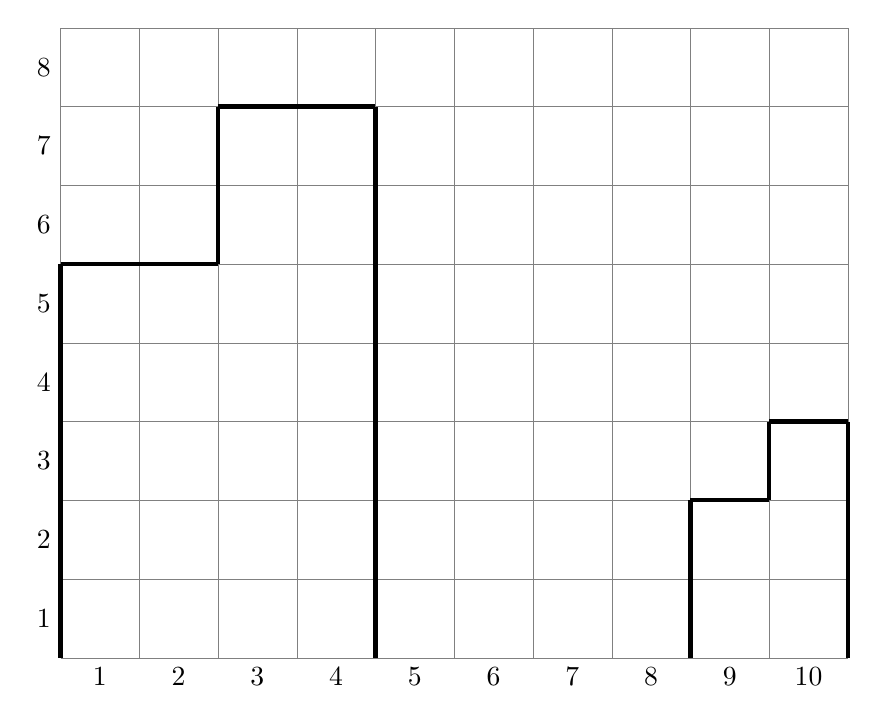
\begin{tikzpicture}
\draw[step=1.0, gray, ultra thin] (0,0) grid (10, 8);

  \draw[ultra thick] (0,0) -- (0, 5);
  \draw[ultra thick] (0, 5) -- (2, 5);
  \draw[ultra thick](2,5) -- (2, 7);
  \draw[ultra thick](2, 7) -- (4, 7);
  \draw[ultra thick](4,7) -- (4, 0);
  \draw[ultra thick](8,0) -- (8, 2);
  \draw[ultra thick](8, 2) -- (9, 2);
  \draw[ultra thick](9, 2) -- (9, 3);
  \draw[ultra thick] (9, 3) -- (10, 3);
  \draw[ultra thick] (10, 3) -- (10, 0);

    \foreach \x in {1, ..., 10} {%
      % Bottom
      \node[anchor=north] at (\x-0.5,0) {\x};
    }
    
    \foreach \y in {1, ..., 8} {%
      % Left
      \node[anchor=east] at (0,\y-0.5) {\y};
    }
\end{tikzpicture}
\newline
\textit{Illustration de l'exemple 1 \\ En noir, là où la ville souhaite poser des panneaux sur les bâtiments.}
\end{figure}

\begin{Input}
	L'entrée consiste de :
	\begin{itemize}
		\item Une ligne avec un entier $n$ ($1 \le n \le 10^4$), la longueur en mètres de la digue.
		\item Une seconde ligne qui représente la ligne d'horizon, composée de $n$ entiers $h_i$ ($0 \le h_i \le 100$) séparés d'un espace représentant la hauteur du bâtiment en position $i$.
	\end{itemize}
\end{Input}

\begin{Output}
	Un entier représentant le nombre de mètres de panneaux nécessaire afin de recouvrir la totalité des côtés et dessus des bâtiments.
\end{Output}

%%% Local Variables:
%%% mode: latex
%%% TeX-master: t
%%% End:
